\chapter{Test and Results}
\label{capitolo4}

\vspace{5cm}

In the first part of the Chapter is tested the correct working of the MONWES library. The test for mirrors, ideal lens and KB is done against OASYS software. For the Montel system, because it is not implemented in OASYS, it is done a benchmark with the paper \cite{resta2015nested}.
\\
The second part of the Chapter use the MONWES library to study the behaviour of the Montel system. It is studied the effect of a non-centred beam watching what happen to the image dimension and the intensity in the case of centred and non centred beam. At the end it is reported the study that I have done, for the beamline ID20 of the ESRF, of a non-orthogonal Montel mirrors.
\vspace{0.5cm}
\section{Testing against OASYS}
%
OASYS (OrAnge SYnchrotron Suite) is a graphical environment for optic simulation used in synchrotron facilities based on orange 3, developped by Manuel Sanchez Del Rio (ESRF) and Luca Rebuffi (ELETTRA).
The comparison between the program and the OASYS software is done with the system in Figure \ref{fig: Optical system}. In this system the 1st optical system collimate the source and the 2nd optical system focalize the Beam at the image plane. The different lentgth that characterize the system are: between the source and the 1st optical system there is a  distance of  $d_1 = f = 0.4 m $, between the 2st and the 2nd optical system a distance $d_2 = 0.6 m $ and the distance between the 2nd system and the image plane correspond to a distance of $d_3 = f = 0.4$. A system that have parameters defined as before, make a copy of the source image at the image plane.
%
\begin{figure}[]
%
\centering
%
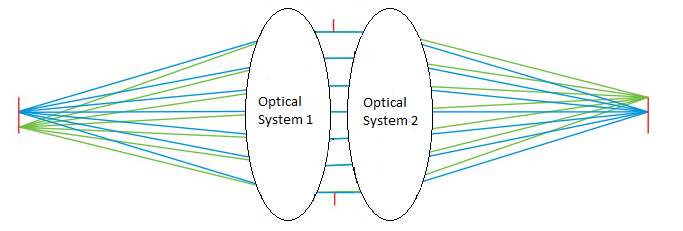
\includegraphics[width=.6\textwidth]{Immagini/Chapter4/OpticalSystems}
%
\caption{Optical system used for the test with OASYS}
%
\label{fig: Optical system}
%
\end{figure}
%
The source parameter used are showed in Figure \ref{fig: Source Parameter for OASYS}, and correspond to  a square source spot of $1 \mu m^2 $, and a initial Gaussian divergence with a FWHM of $2.3 mrad $.
\begin{figure}[]
%
\centering
%
\subfloat[][Initial spot size \label{fig: Source OASYS}]
   {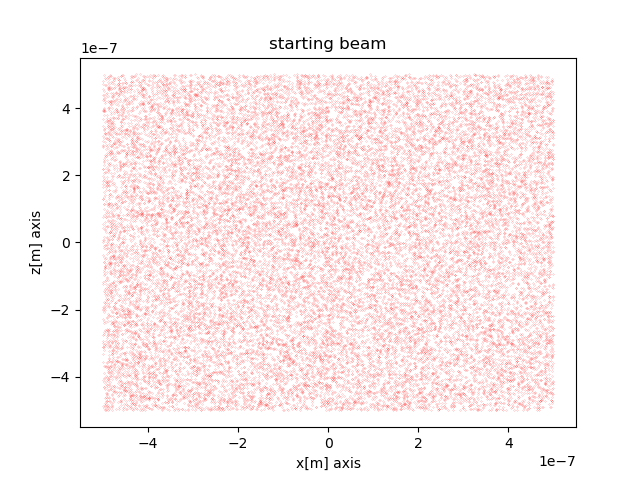
\includegraphics[width=.4\textwidth]{Immagini/Chapter4/SouceOASYS}}
%
\subfloat[][Initial Beam divergence\label{fig: Divergence OASYS}]
   {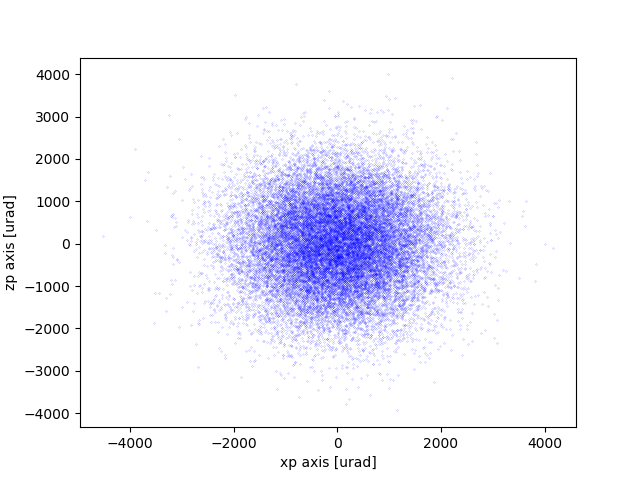
\includegraphics[width=.48\textwidth]{Immagini/Chapter4/DivergenceOASYS}}
%
\caption{Parameter of the source used for the test with OASYS}
%
\label{fig: Source Parameter for OASYS}
%
\end{figure}
%
The tests is done using different optical system, with the same focal length and, for the mirror, with a grazing incidence angle of $\theta = 1.719^{\circ}$. Below are plotted the image of the Beam at the image plane, putting the OASYS results on the right, and my results on the left. 
\\
The system simulated are done with:
\begin{enumerate}
\item ideal lenses Figure \ref{fig: Ideal lense OASYS}
\item parabolic mirror Figure \ref{fig: paraboloid OASYS}
\item KB system Figure \ref{fig: KB system OASYS}
\end{enumerate} 
\noindent As it is showed in the figures \ref{fig: Ideal lense OASYS}, \ref{fig: paraboloid OASYS} and KB system Figure \ref{fig: KB system OASYS}, the result, of OASYS and my simulations are in good agreement. The ideal lenses case show a perfect replica of the source image, on the contrary, KB and paraboloid, show similar images but a bit aberrated, because it degrades along the propagation.
\newpage
%
\begin{figure}[H]
%
\centering
%
\subfloat[][My ideal lenses simulation \label{fig: my Ideal Lenses}]
   {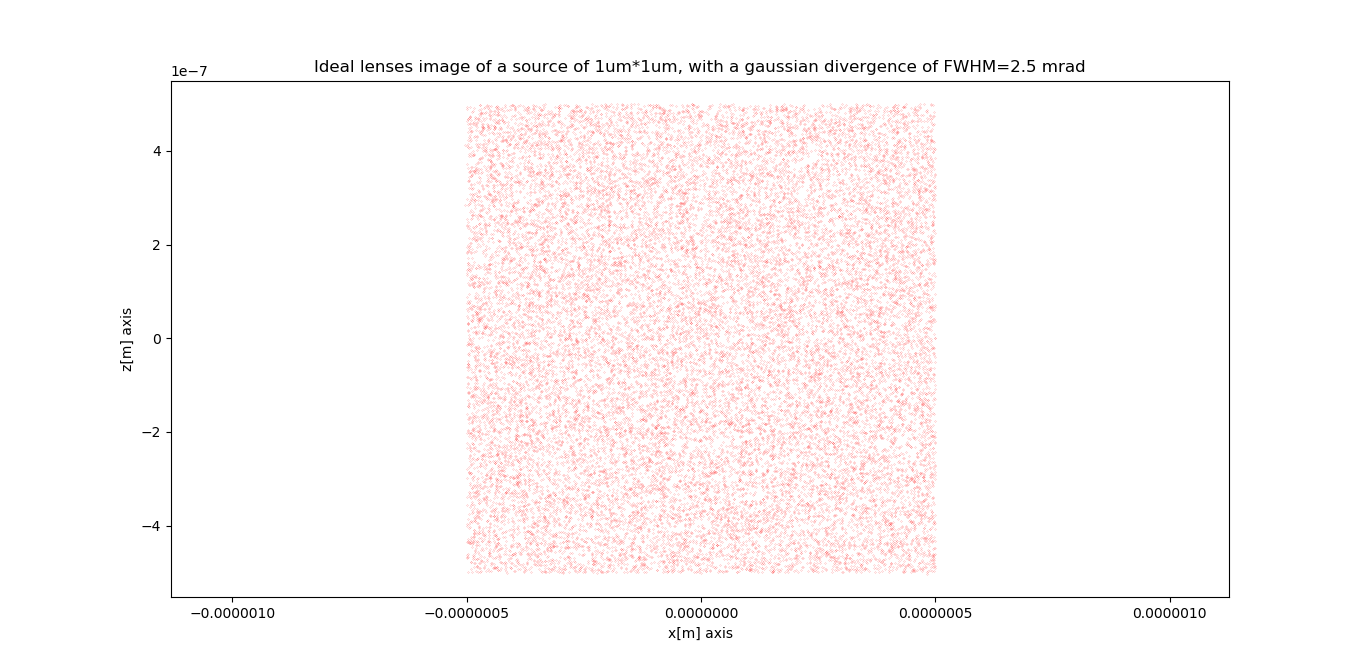
\includegraphics[width=.5\textwidth]{Immagini/Chapter4/IdealLens}}
%
\subfloat[][OASYS ideal lenses simulation \label{fig: Ideal Lenses OASYS}]
   {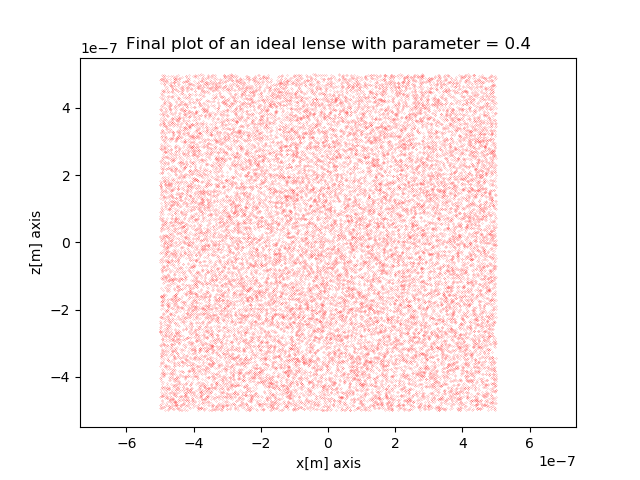
\includegraphics[width=.5\textwidth]{Immagini/Chapter4/IdealLensOASYS}}
%
\caption{Image for the testing ideal lenses system in Figure \ref{fig: Optical system} of: my simulation (Figure \ref{fig: my Ideal Lenses}) and OASYS simulation (Figure \ref{fig: Ideal Lenses OASYS})}
%
\label{fig: Ideal lense OASYS}
%
\end{figure}
%
\begin{figure}[H]
%
\centering
%
\subfloat[][My paraboloid simulation \label{fig: my Paraboloid}]
   {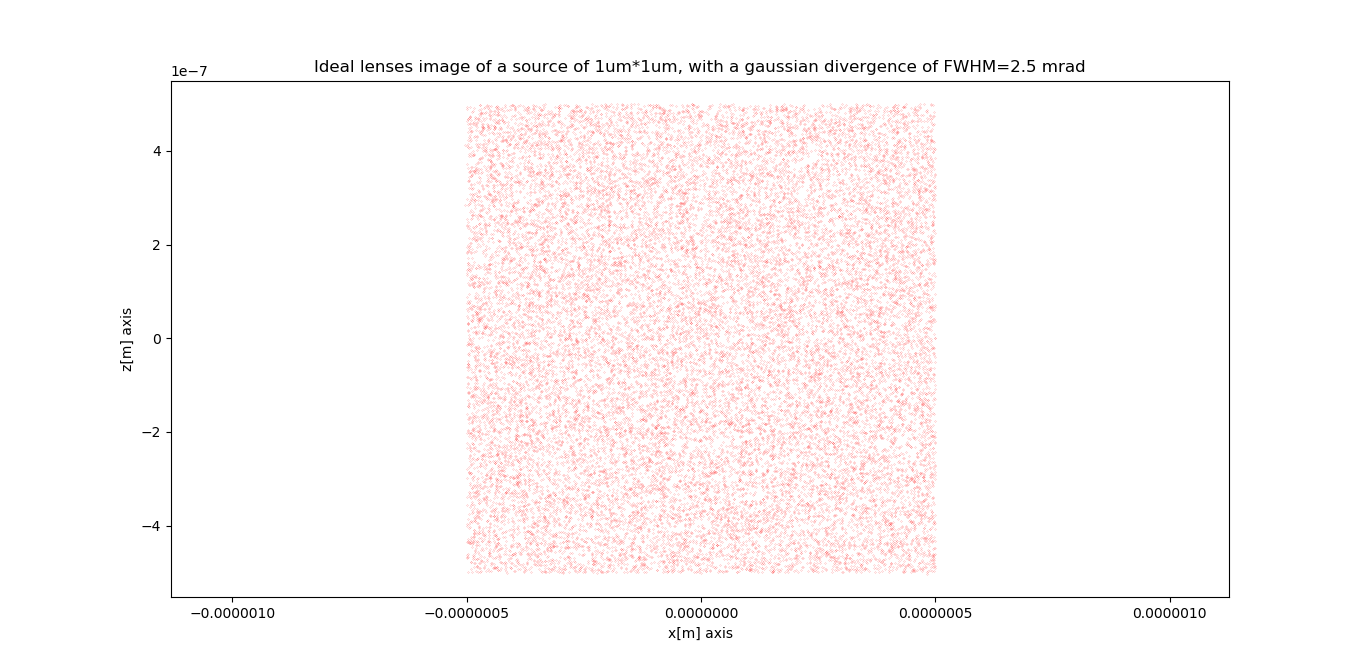
\includegraphics[width=.5\textwidth]{Immagini/Chapter4/IdealLens}}
%
\subfloat[][OASYS paraboloid simulation \label{fig: Paraboloid OASYS}]
   {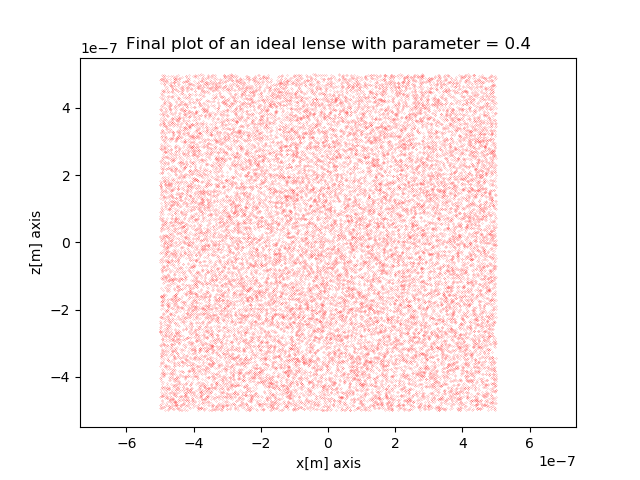
\includegraphics[width=.5\textwidth]{Immagini/Chapter4/IdealLensOASYS}}
%
\caption{Image for the testing paraboloid system in Figure \ref{fig: Optical system} of: my simulation (Figure \ref{fig: my Paraboloid}) and OASYS simulation (Figure \ref{fig: Paraboloid OASYS})}
%
\label{fig: paraboloid OASYS}
%
\end{figure}
%
\begin{figure}[H]
%
\subfloat[][My KB simulation \label{fig: my KB}]
   {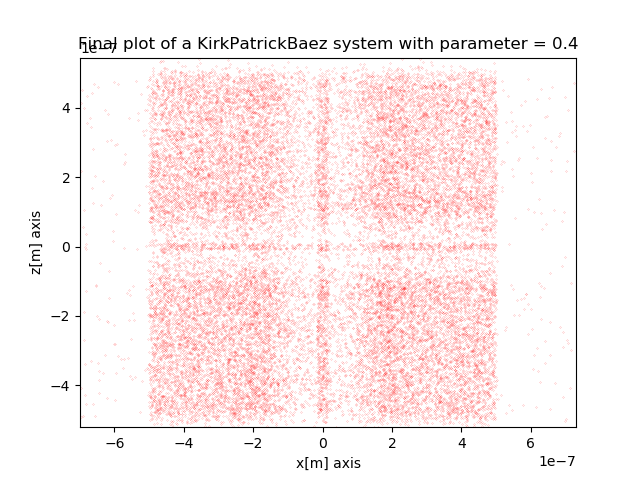
\includegraphics[width=.5\textwidth]{Immagini/Chapter4/KB}}
%
\subfloat[][OASYS KB divergence\label{fig: KB OASYS}]
   {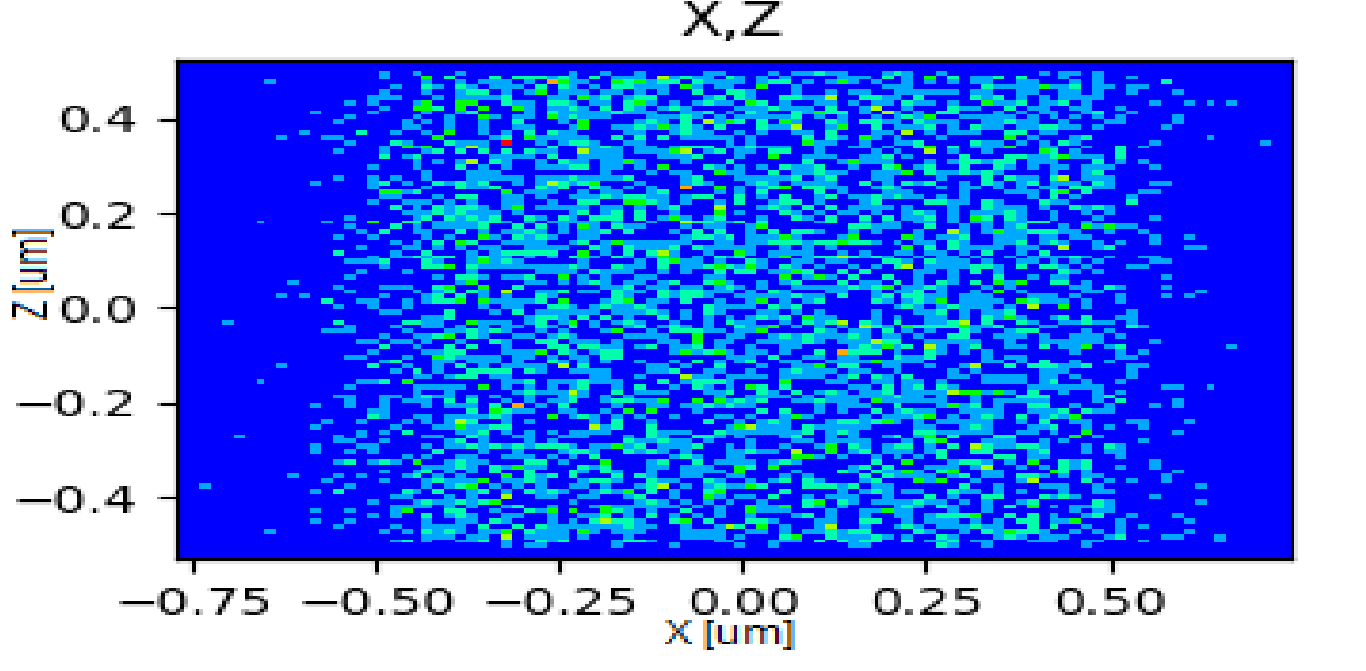
\includegraphics[width=.5\textwidth]{Immagini/Chapter4/KBOASYS}}
%
\caption{Image for the testing KB system in Figure \ref{fig: Optical system} of: my simulation (Figure \ref{fig: my KB}) and OASYS simulation (Figure \ref{fig: KB OASYS})}
%
\label{fig: KB system OASYS}
%
\end{figure}
%
\newpage
%
\subsection{Benchmarking} 
The system used for the benchmarking is showed in Figure \ref{fig: PaperMontelSystem} using the reference frame of the paper \cite{resta2015nested}. The aim of this system is to collimate a Beam using a Montel with two parabolic mirrors. The source used has a Gaussian dimension of 2.5$\mu $m FWHM and a Gaussian divergence of 5$mrad $. The distances, between the source/image plane and the center of the Montel are, respectively,  $\simeq $ 0.26m and 10.06m. The incidence angle of the Beam is $\theta_g \simeq 2.86^{\circ} $.
%
\begin{figure}[]
	\centering
		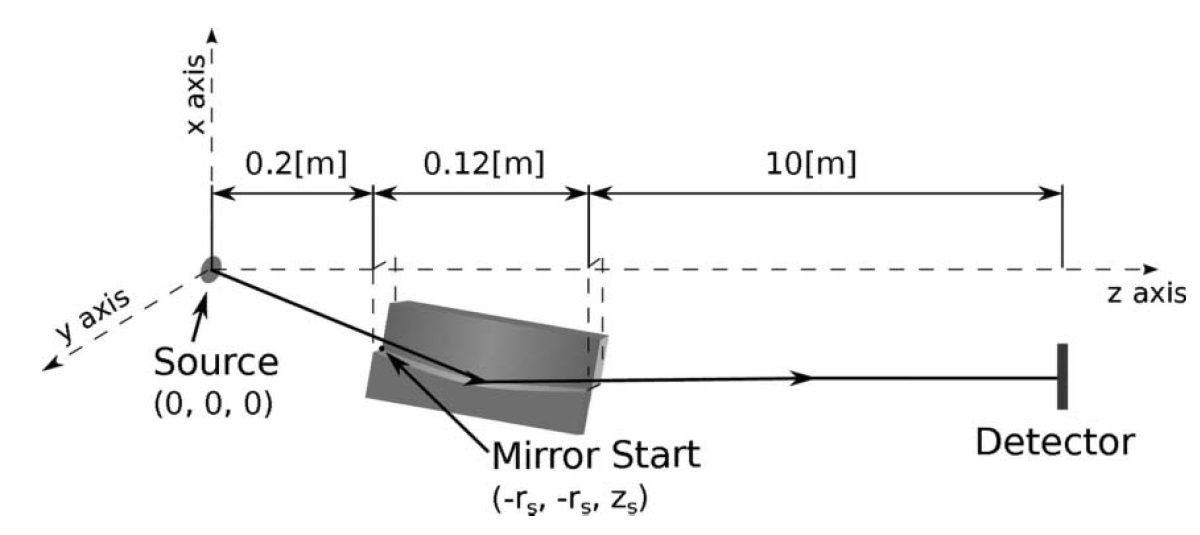
\includegraphics[width=0.8\textwidth]{Immagini/Chapter4/PaperMontelSystem}
		\caption{Illustration of the Montel system used as a collimator in the paper \cite{resta2015nested}}
		\label{fig: PaperMontelSystem}
\end{figure}
%
The result, at the image plane, of the beam size and beam divergence, after the double-reflection of the Montel system, is showed in Figure \ref{fig: My Simulation Comparison}. There in Figure \ref{fig: PaperImageShape} shows the beam at the image plane, and  Figure \ref{fig: PaperImageDivergence}shows the divergence. The quantitative values reported on the paper correspond to a Gaussian-like distribution with a spatial FWHM of $\sim $0.7mm for the spot size, and a FWHM of the Gaussian divergence $\sim $ 0.01 mrad.
\\
Repeating the simulation with MONWES, and using the parameter defined in  in the paper \cite{resta2015nested} it obtain Figure \ref{fig: My Simulation Comparison}. As it is showed in the Figure \ref{fig: My Simulation Comparison} there are a qualitative good agreement between the two simulation. Also, under a quantitative point of view, there is a good agreement in fact, in my simulation are obtained a value of $\sim $1mm of FWHM of image size, pretty similar to the one of the other simulation, and $\sim $0.01 mrad FWHM of divergence that is equal to the one obtained with the other simulation.
%
\begin{figure}[]
%
\centering
%
\subfloat[][Beam image shape of the paper\label{fig: PaperImageShape}]
   {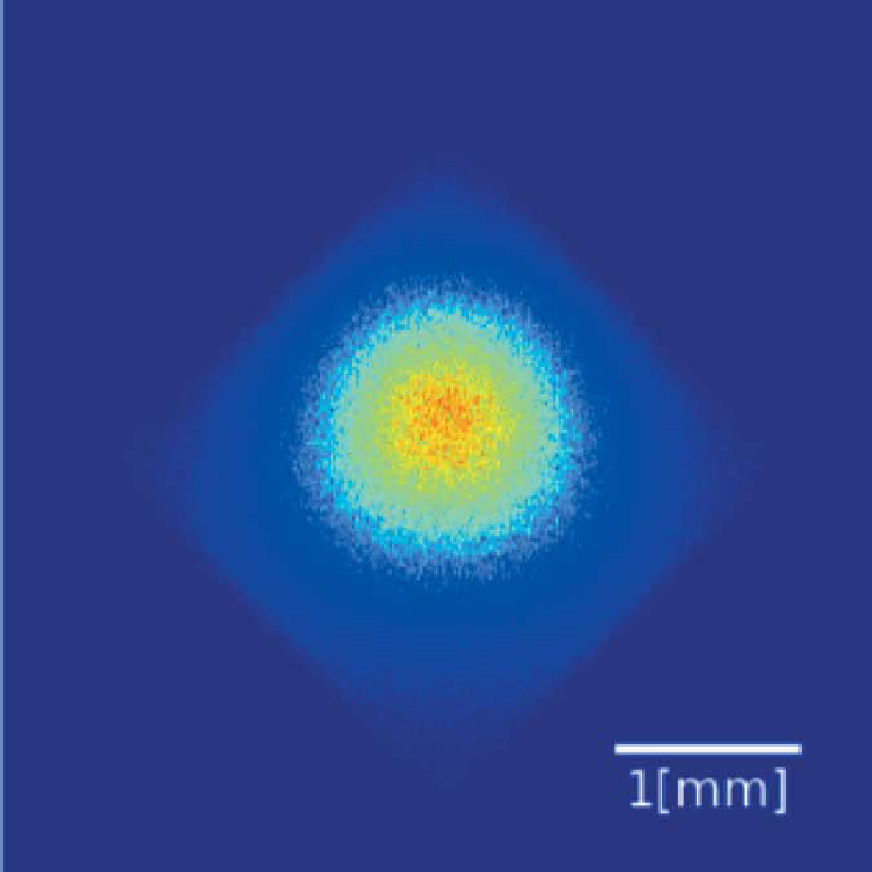
\includegraphics[width=.4\textwidth]{Immagini/Chapter4/PaperSpotMontel}}
%
\subfloat[][Beam image shape of the simulation\label{fig: Image dimension}]
   {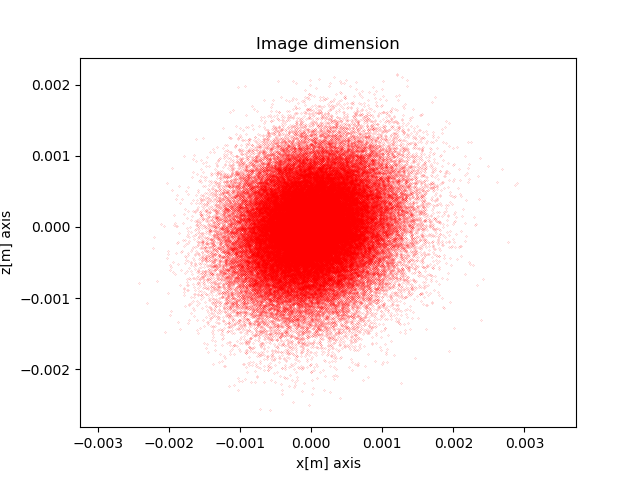
\includegraphics[width=.48\textwidth]{Immagini/Chapter4/ImageDimension}}\quad
%
\subfloat[][Beam image divergence of the paper\label{fig: PaperImageDivergence}]
   {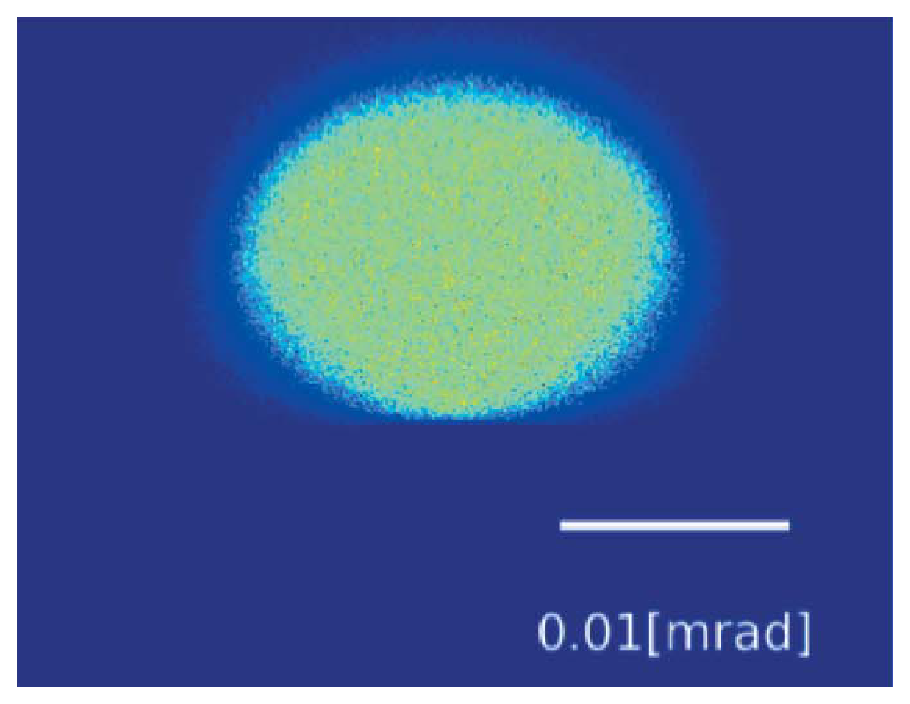
\includegraphics[width=.4\textwidth]{Immagini/Chapter4/PaperDivergenceMontel}}
%
\subfloat[][Beam image divergence of the simulation\label{fig: Divergence dimension}]
   {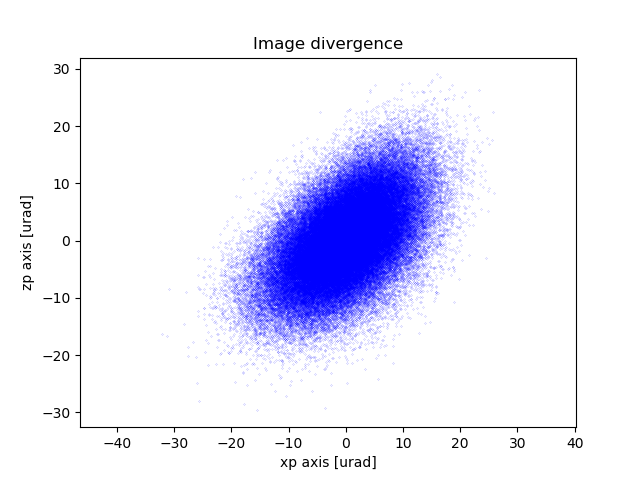
\includegraphics[width=.48\textwidth]{Immagini/Chapter4/DivergenceDimension}}
%
\caption{Results of  the Montel simulations with a source beam with a FWHM spot of 2.5$\mu $m and a Gaussian divergence of 5$mrad $}
%
\label{fig: My Simulation Comparison}
%
\end{figure}
%
\section{Analysis of Montel system}
In this section a study of the Montel is done, using the Montel tools developed. The first simulation, to verify that Montel work well, study the behaviour of a point-wise source with a certain divergence, using a collimating system. The second simulation, for the same reason of before, simulates a collimating beam with a certain source shape geometry and figure out the image plot obtained by a focalizing system in its image plane. What is expected is a point in the divergence space for the first situation and in the real space for the second simulation, as a consequence of the ideal collimating/focalizing system. For the simulation parabolic Montel with an incidence angle of 2$^{\circ} $ (the choice of the angle is arbitrary) are used. Paraboic system are chosen because is the only way to obtain a perfect collimating Beam.
\\
Figure \ref{fig: ideal} reports the result for the ideal collimating/focalizing cases.
For the collimation system a point wise source  is used with a Gaussian divergence of FWHM of 25$\mu $m, \ref{fig: coll.Source}. At the image plane the Beam (Figure \ref{fig: CollimationImage}) is collimated, reducing its divergence of 3 orders of magnitude. For the focalizing system, it is used a circular source spot having a radius of 1mm, Figure \ref{fig: foc.Source}, with a collimated source beam. At the image plane the dimension of the Beam (Figure \ref{fig: focalizingImage}) is reduced of 3 order magnitude. It is possible to conclude that both collimating and focalizing system work but not perfectly (the final results are not point). One explanation can be that, because of the particular configuration of the mirrors of the Montel, the effect on the Beam are not perfect. This can be an \textbf{intrinsic aberration of the Montel}, that can be studied more in the future.
\\
\begin{figure}[]
%
\centering
%
\subfloat[][Source divergence\label{fig: coll.Source}]
   {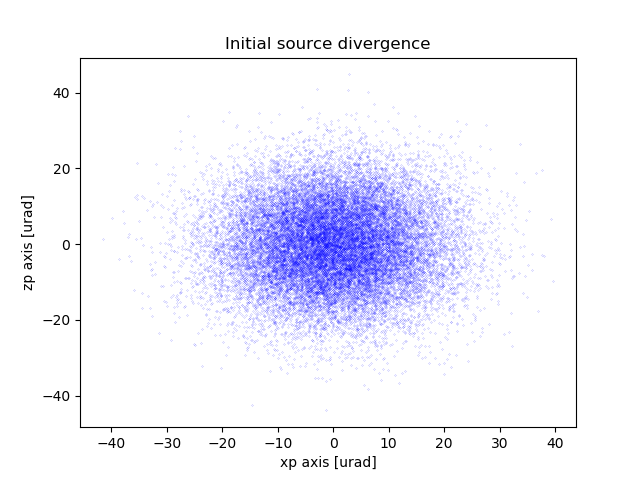
\includegraphics[width=.4\textwidth]{Immagini/Chapter4/CollimationSource}}
%
\subfloat[][Image divergence\label{fig: CollimationImage}]
   {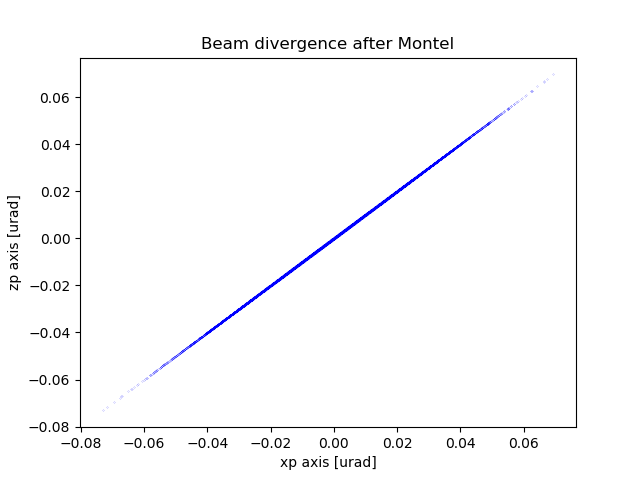
\includegraphics[width=.4\textwidth]{Immagini/Chapter4/CollimationImage}}\quad
%
\subfloat[][Source divergence\label{fig: foc.Source}]
   {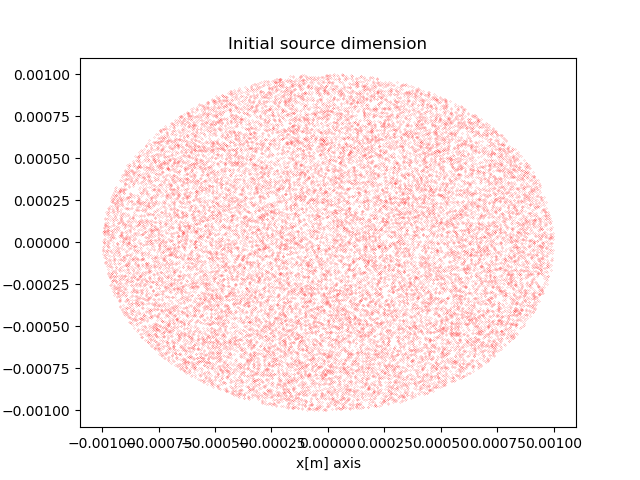
\includegraphics[width=.4\textwidth]{Immagini/Chapter4/FocalizingSource}}
%
\subfloat[][Image divergence\label{fig: focalizingImage}]
   {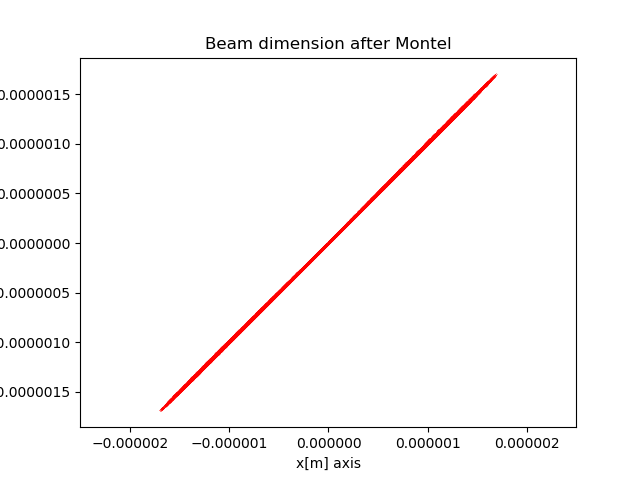
\includegraphics[width=.4\textwidth]{Immagini/Chapter4/FocalizingImage}}
%
\caption{Ideal system}
%
\label{fig: ideal}
%
\end{figure}
%
Up to now the dimension of the Montel were not considered. The Montel is set to have infinite dimension in all the direction. This approach hold in the case of a small source and a narrow profile divergence, that hit only a small part of the system. Otherwise, for example of an isotropic source that can be modelled with a very big divergence, the situation change. In this part, to study to behaviour of a big source, it is used a Beam source with a square shape with a side of 1mm, with a Gaussian profile divergence of FWHM=1mrad. These parameter show what happen to the Montel where it is covered over all its surface. I  this case a focalizing parabolic Montel is used with:  object  distance of 1m, image distance of 3m, incidence angle of $2^{\circ} $,  length of the Monte of 0.1m and width of the Montel of 20cm.
%
\begin{figure}[]
%
\centering
%
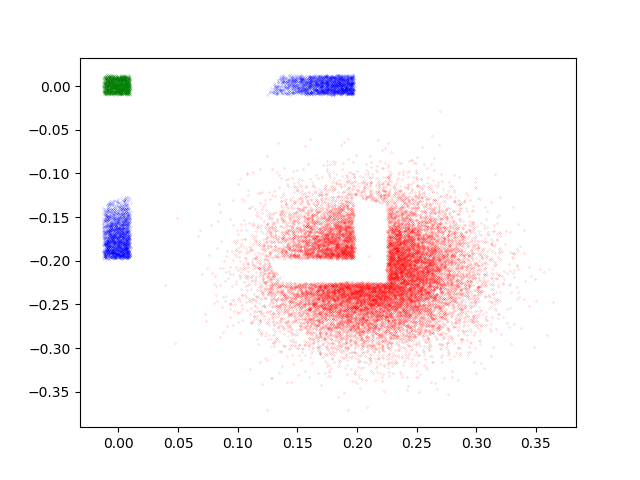
\includegraphics[width=.6\textwidth]{Immagini/Chapter4/BigSourceMontel}
%
\caption{Illumination at the image plane of the different Beam (red dots correspond to np-reflected rays, blue dot to one-reflected rays, green dots to two-reflected rays).}
%
\label{fig:BigSourceMontel}
%
\end{figure}
%
Figure \ref{fig:BigSourceMontel}, show thee image plane of the Montel defined above. This plot show 4 figure, the biggest one, represented by the red dots, correspond to the rays that reach the image plane without touch the Montel, the rays coloured in blue, are those which are subject to only one reflection that are positioned in different part of the image plane depending which mirror meet, those that hit the xy-mirror correspond to the beam elongated along z, the zy-mirror correspond to the beam elongate along x. At the end, the green dots, are the rays that do both reflection and are centred to the center of the image plane by definition of it.


\section{Non-centred Beam}
In this section is studied the effect of a Montel system of a non centred-Beam in order to understand how to align correctly beam. The alignment study is study simulating a beam tha hit different point of the Montel. Is reported the behaviour about the change of FWHM of both $x^{'} $ and $z^{'} $, of a small ($1 \mu m^2 $) source with a narrow divergence ($25 \mu rad $), following different path. Figure \ref{fig: path} show the different path followed to simulate the non-centred. Every path is labelled with a name:
\begin{enumerate}
	\item Y
	\item XZ
	\item XYZ1
	\item XZY2
\end{enumerate}

\begin{figure}[]
%
\centering
%
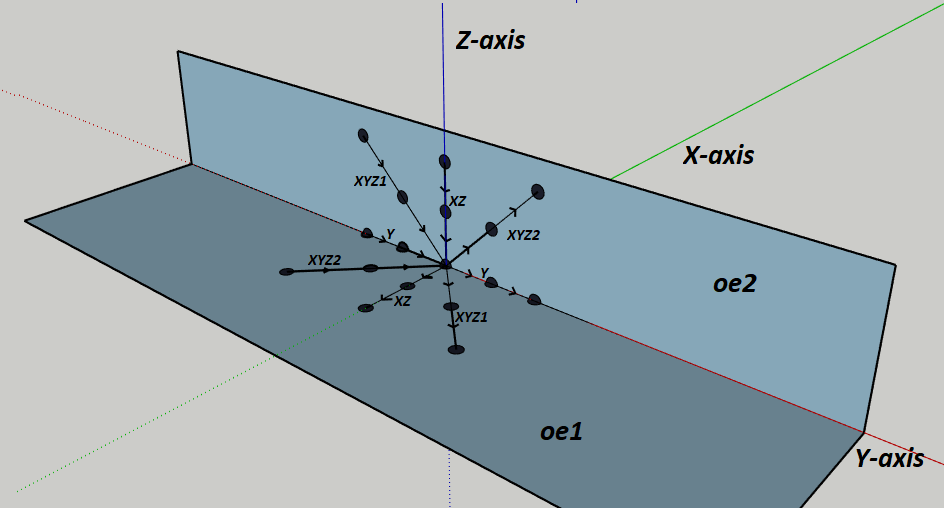
\includegraphics[width=1.\textwidth]{Immagini/Chapter4/Cattura2}
%
\caption{Different path for simulate the non-centred beam}
%
\label{fig: path}
%
\end{figure}

The system used is a focalizing parabolic Montel with an object focal distance of 0.2m and an image focal distance of 0.9, working on miroor designe for incidence angle of $\theta_g = 2^{\circ}$. Figure \ref{fig: reuslt diff. path} show the result the two FWHM of the beam changing the incidence point of the beam moving the different paths. This point is defined with respect to the center of the Montel system that correspond to the origin (0, 0, 0). In Figure \ref{fig: Y path}, the incidence point move along y-axis, start from the point (0, 1.5mm, 0) and arriving to the point (0, -1.5mm, 0), and show, more or less, a flat behaviour of the FWHM. Figure \ref{fig: XZ path} start from the point (0, 0, 0.15mm) and arrive to (-0.15mm, 0, 0) and have specular behaviour for the two FWHM, there is a minimum of the two FWHM near the origin point, moving on the oe1 worse the FWHM of $z^{'} $ and maintain the other constant, on the contrary, moving on the oe2 the situation is reversed, in this case the FWHM of $x^{'} $ get worse, maintaining constant the one of $z^{'} $. Figure \ref{fig: XYZ1 path} start from (0, 1.5mm, 0.15mm) and arrive to (-0.15mm, -1.5mm, 0) and Figure \ref{fig: XYZ2 path} start from (-0.15mm, 1.5mm, 0) and arrive to (0., -1.5mm, 0.15mm). The behaviour of this last two path are similar to that of \ref{fig: XZ path}, this is reasonable, because the motion along y-axis does not influence the FWHM because of the definition of the cylindrical mirror, that in any point along the y direction have the same geometry.
\\
%
%
\begin{figure}[]
%
\centering
%
\subfloat[][Y path\label{fig: Y path}]
   {\includegraphics[width=.4\textwidth]{Immagini/Chapter4/Ypath}}
%
\subfloat[][XZ path\label{fig: XZ path}]
   {\includegraphics[width=.4\textwidth]{Immagini/Chapter4/XZpath}}\quad
%
\subfloat[][XYZ1 path\label{fig: XYZ1 path}]
   {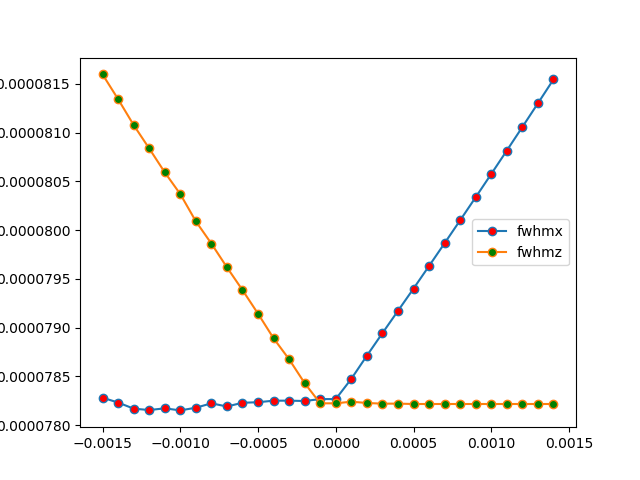
\includegraphics[width=.4\textwidth]{Immagini/Chapter4/XYZ1Path}}
%
\subfloat[][XYZ2 path\label{fig: XYZ2 path}]
   {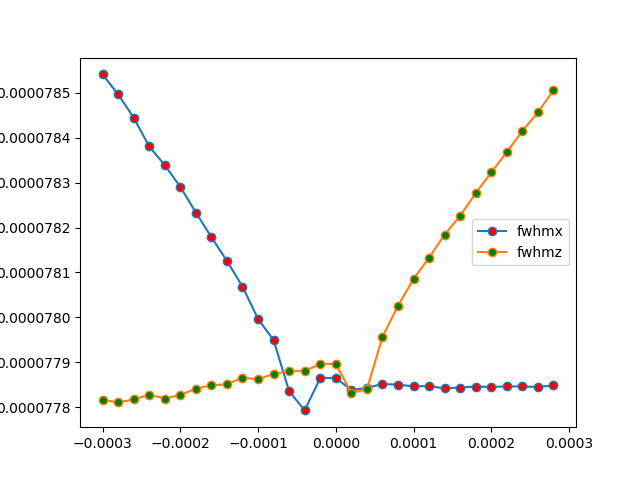
\includegraphics[width=.4\textwidth]{Immagini/Chapter4/XYZ2Path}}
\caption{Results of the changing of the x and z FWHM at the image following different path defined in Figure \ref{fig: path}. The Montel system used have a source beam with a FWHM spot of 2.5$\mu $m and a Gaussian divergence of 5$mrad $}
%
\label{fig: reuslt diff. path}
%
\end{figure}
In Figure \ref{fig: 2nd reuslt diff. path} it is show the intensity profile of the two-reflection beam of source with a $10 mm^2 $ of area and a Gaussian divergence of FWHM = $25 \mu rad $. In this case the Montel used is the same as before but with a length of 20cm and a width of 2cm.  The intensity is calculated as the number of the rays in the two-reflection beam with respect to the initial number of rays. 
The different path move along these points; ymax=50cm, ymin=-50cm, xmin=-2cm, xmax=0, zmax=2cm, zmin=0
\\
The plots in Figure \ref{fig: 2nd reuslt diff. path}, are interesting, because represents the intensity of the "green" Beam in Figure \ref{fig:BigSourceMontel}, that can be directly measured and so, it is possible to relate the centring of the Beam calculating the intensity of this Beam.
%
\begin{figure}[]
%
\centering
%
\subfloat[][Y path\label{fig: Y path}]
   {\includegraphics[width=.4\textwidth]{Immagini/Chapter4/Ypath_2}}
%
\subfloat[][XZ path\label{fig: XZ path}]
   {\includegraphics[width=.4\textwidth]{Immagini/Chapter4/XZpath_2}}\quad
%
\subfloat[][XYZ1 path\label{fig: XYZ1 path}]
   {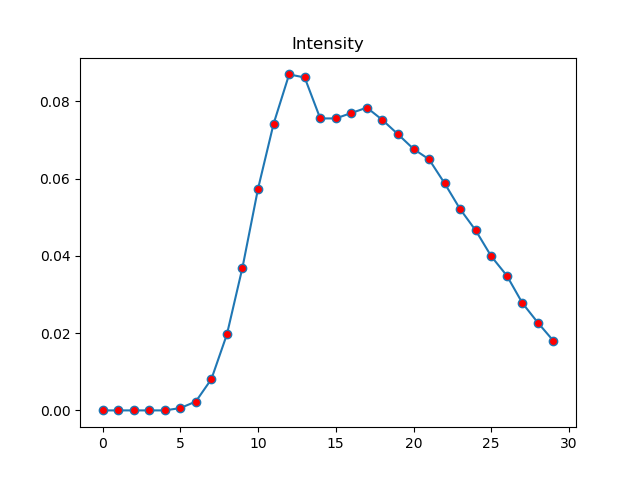
\includegraphics[width=.4\textwidth]{Immagini/Chapter4/XYZ1Path_2}}
%
\subfloat[][XYZ2 path\label{fig: XYZ2 path}]
   {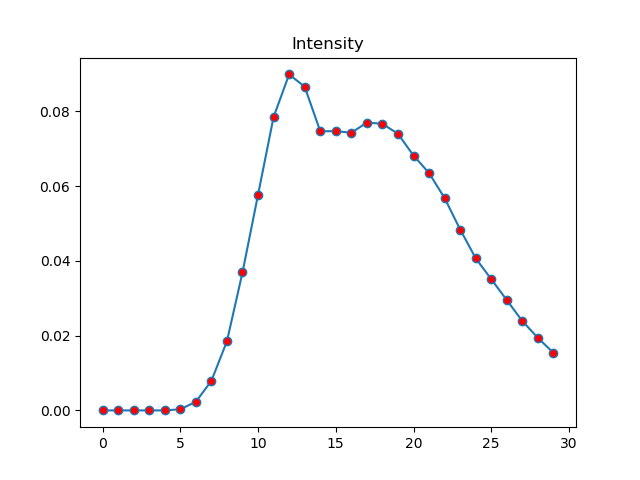
\includegraphics[width=.4\textwidth]{Immagini/Chapter4/XYZ2Path_2}}
\caption{Change of the intensity depending on the path defined in Figure \ref{fig: path}. The Montel system used have a square spot of $10 mm^2 $ and a Gaussian divergence of $25mrad $}
%
\label{fig: 2nd reuslt diff. path}
%
\end{figure}
\section{Simulation of a Montel system for ID20}

In this section is reported the study that I have done for the beam of ID20 of the ESRF. The simulation were done in order to study the Montel system bought as analyser that will be used in the beamline.

\subsection{System parameters}
The system simulated have a source size of $ 1 \mu m^2 $(see Figure \ref{fig: ID20InitialSpot}) with a Gaussian divergence of $25 \mu rad $(see Figure \ref{fig: ID20InitialDivergence}). The parameters of the system are: object distance of $351 mm$, mirror Length of $300mm$, mirror width of $100mm $, the error max between the orthogonal configuration of the two mirror is of $\Delta =  \pm 0.03^{\circ} $ and an incidence angle of $18.1 mrad $. In Figure \ref{fig: ID20System} is showed a 3D graphic view of the Monter system with the parameter used.
\begin{figure}[H]
%
\centering
%
\subfloat[][Beam source size (1$\mu $ $m^2 $)\label{fig: ID20InitialSpot}]
   {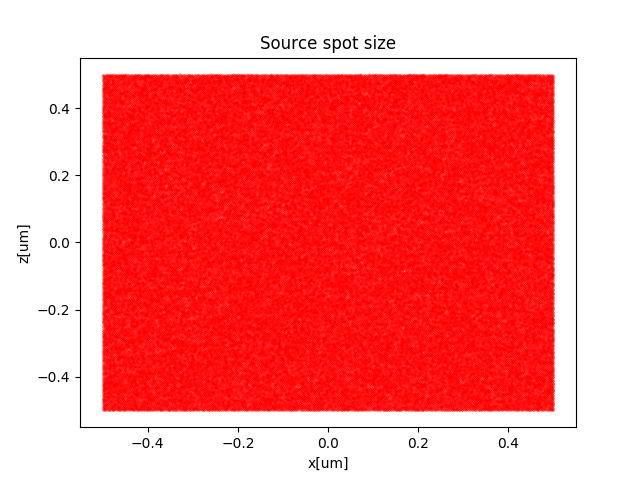
\includegraphics[width=.4\textwidth]{Immagini/Chapter4/ID20InitialSpot}}
%
\subfloat[][Beam source divergence ($2h \mu $ $rad $)\label{fig: ID20InitialDivergence}]
   {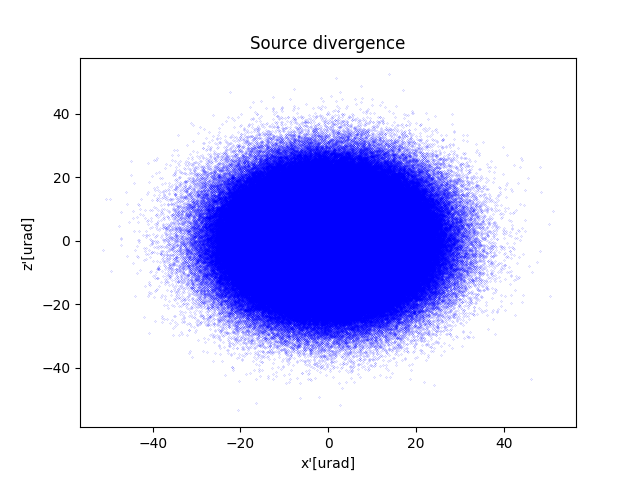
\includegraphics[width=.4\textwidth]{Immagini/Chapter4/ID20InitialDivergence}}\quad
%
\caption{Source parameters used for the study of the Montel Analyser for ID20}
%
\end{figure}

\begin{figure}[H]
%
\centering
%
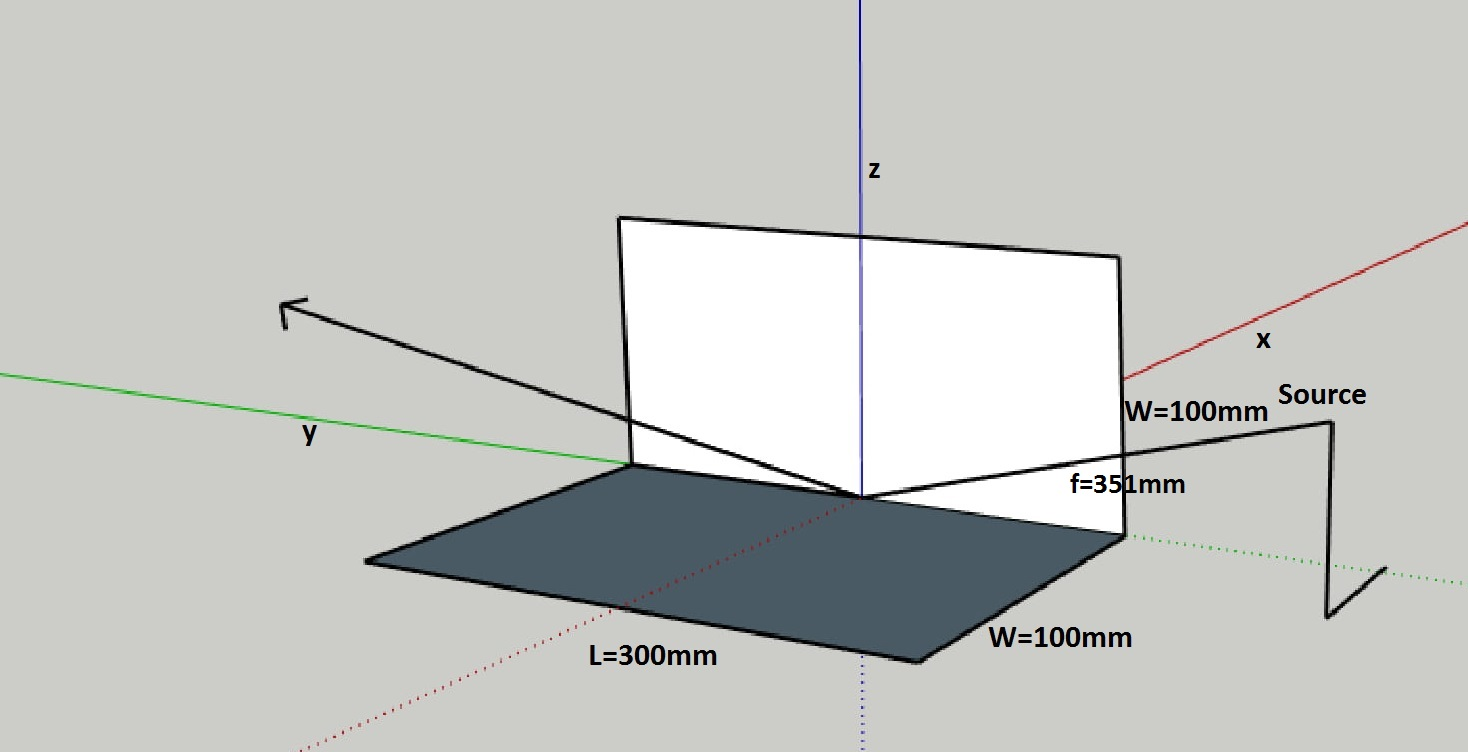
\includegraphics[width=1.\textwidth]{Immagini/Chapter4/ID20System}
%
\caption{Montel parameters used for the simulation for ID20}
%
\label{fig: ID20System}
%
\end{figure}

\subsection{Result of beam figure and footprint}

The image plane is positioned at $1m$ from the center of the Montel system. The property of the beam at the image plane are showed in Figure \ref{fig: ID20image}.It is obtained, a new spot size with a length of $60 \mu $ $m$ in the x direction and $100 \mu $ $m$ in the z direction, and the divergence has a dimension of $\simeq 40\mu$ $rad$.
\begin{figure}[H]
%
\centering
%
\subfloat[][Size of the Beam at the image plane\label{fig: image_spot}]
   {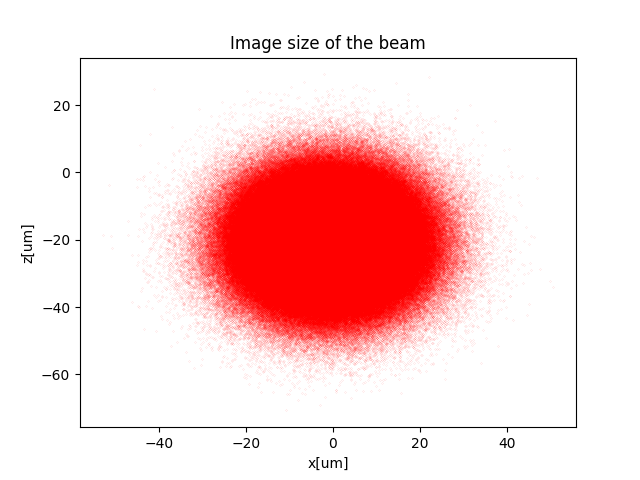
\includegraphics[width=.4\textwidth]{Immagini/Chapter4/image_spot}}
%
\subfloat[][Divergence of the Beam at the image plane\label{fig: image_divergence}]
   {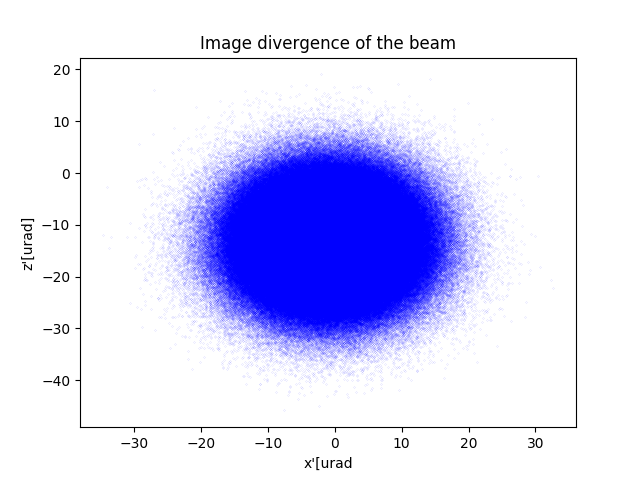
\includegraphics[width=.4\textwidth]{Immagini/Chapter4/image_divergence}}\quad
%
\label{fig: ID20image}
%
\end{figure}
\noindent Moreover is interesting to note the footprint of the two mirror (Figure \ref{fig: footprint}) because the area hit by the beam have a greater component on the y direction (due to the grazing incidence), than in the other direction.The x-length of the xy-mirror, and the z-length of the zy-mirror, is very small (at the order of $20 \mu $ $m$) with respect to the y-length that is $\simeq 20mm$.
%
\begin{figure}[H]
%
\centering
%
\subfloat[][Footprint on oe1\label{fig: footprint_oe1}]
   {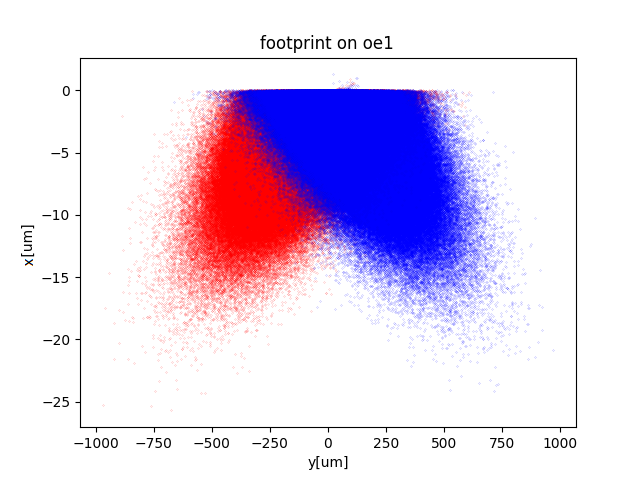
\includegraphics[width=.4\textwidth]{Immagini/Chapter4/footprint_oe1}}
%
\subfloat[][Footprint on oe2\label{fig: footprint_oe2}]
   {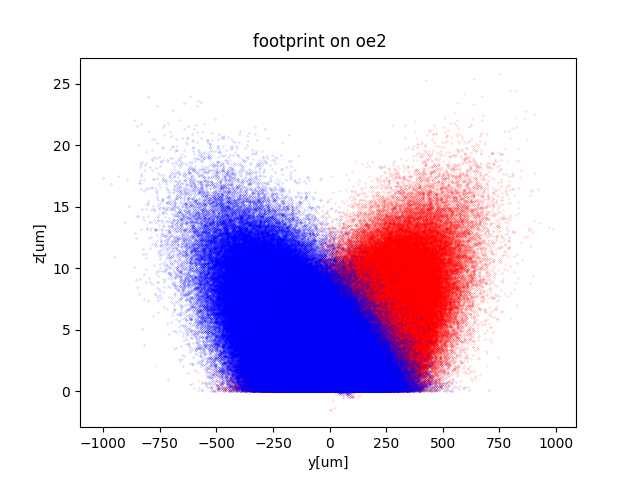
\includegraphics[width=.4\textwidth]{Immagini/Chapter4/footprint_oe2}}\quad
%
\caption{Footprint, on the xy-mirror (\ref{fig: footprint_oe1}) and on zy-mirror (\ref{fig: footprint_oe2}). The red dots are those rays that hit before xy-mirror and after zy-mirror, the blue ones hit first xy-mirror and after zy-mirror.}
%
\label{fig: footprint}
%
\end{figure}
\subsection{Analysis of orthogonality}
Figure \ref{fig: Histogram} presents the interesting histograms versus the horizontal anlge $x^{’} $ when the angle between the mirrors change ($\alpha = 90^{\circ} + \Delta $). It can be noted a improvement of the collimation of the beam changing the angle in the case of closer mirrors ($\Delta=-0.01^{\circ} $
). Figure \ref{fig:FWHM changing orthogonality} show the trend of the FWHM of the $x^{'} $ changing the angle $\Delta $, it is possible to note a minimum for negative angle (this ideal situation is the pink curve reported in Figure \ref{fig: Histogram}) after that the situation become worse. Moreover, the behavior of the FWHM is not symmetrical with respect to $0^{\circ} $, in case of negative angle deviation the situation improve for a small range of deviation angle, after that, the trend get worse, on the opposite way, the situation get worse increasing the positive
deviation angle.

\begin{figure}
%
\centering
%
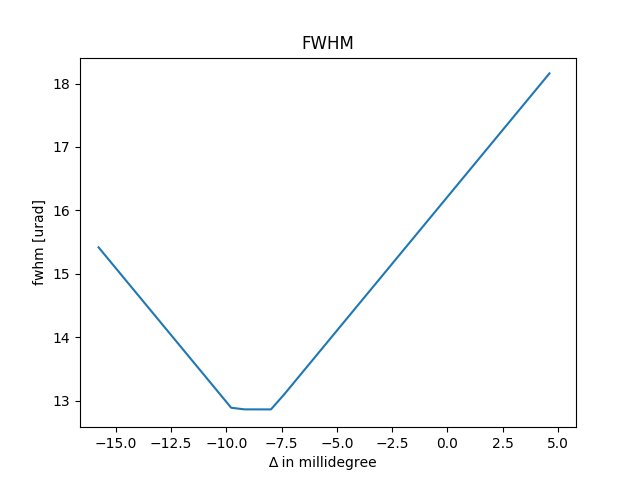
\includegraphics[width=.68\textwidth]{Immagini/Chapter4/FWHM}
%
\caption{FWHM of x' after the Montel changing the orthogonality}
%
\label{fig:FWHM changing orthogonality}
%
\end{figure}
\begin{figure}[]
%
\centering
%
\subfloat[][Real histogram\label{fig:HistogramFitted2}]
   {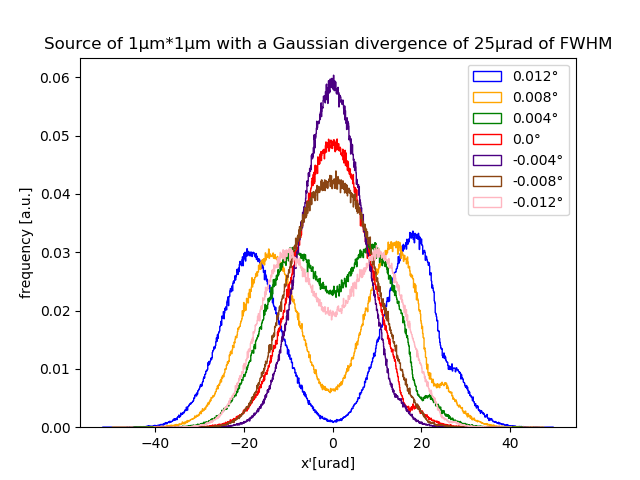
\includegraphics[width=0.6\textwidth]{Immagini/Chapter4/Histogram}}\quad
%
\subfloat[][Fitted Histogram\label{fig:HistogramFitted}]
   {\includegraphics[width=.7\textwidth]{Immagini/Chapter4/Histogram2}}
%
\caption{Histogram of x' after Montel}
%
\label{fig: Histogram}
%
\end{figure}
